\section{Development}

\subsection*{3.1 Peripherals integration}



Doing experiments we discovered that the frequency of the pump machine internal motors was
creating an interference in the flowrate. Therefore compromising the stabilization in cone jet mode.
A solution for that was to increase the flowrate wich smooths this pumping noise. For that was also necessary
to increase the nozzle diameter to balance with all other variables from the experiment.


\subsection*{3.2 Experiment 1}

\begin{figure}[H]
    \center
    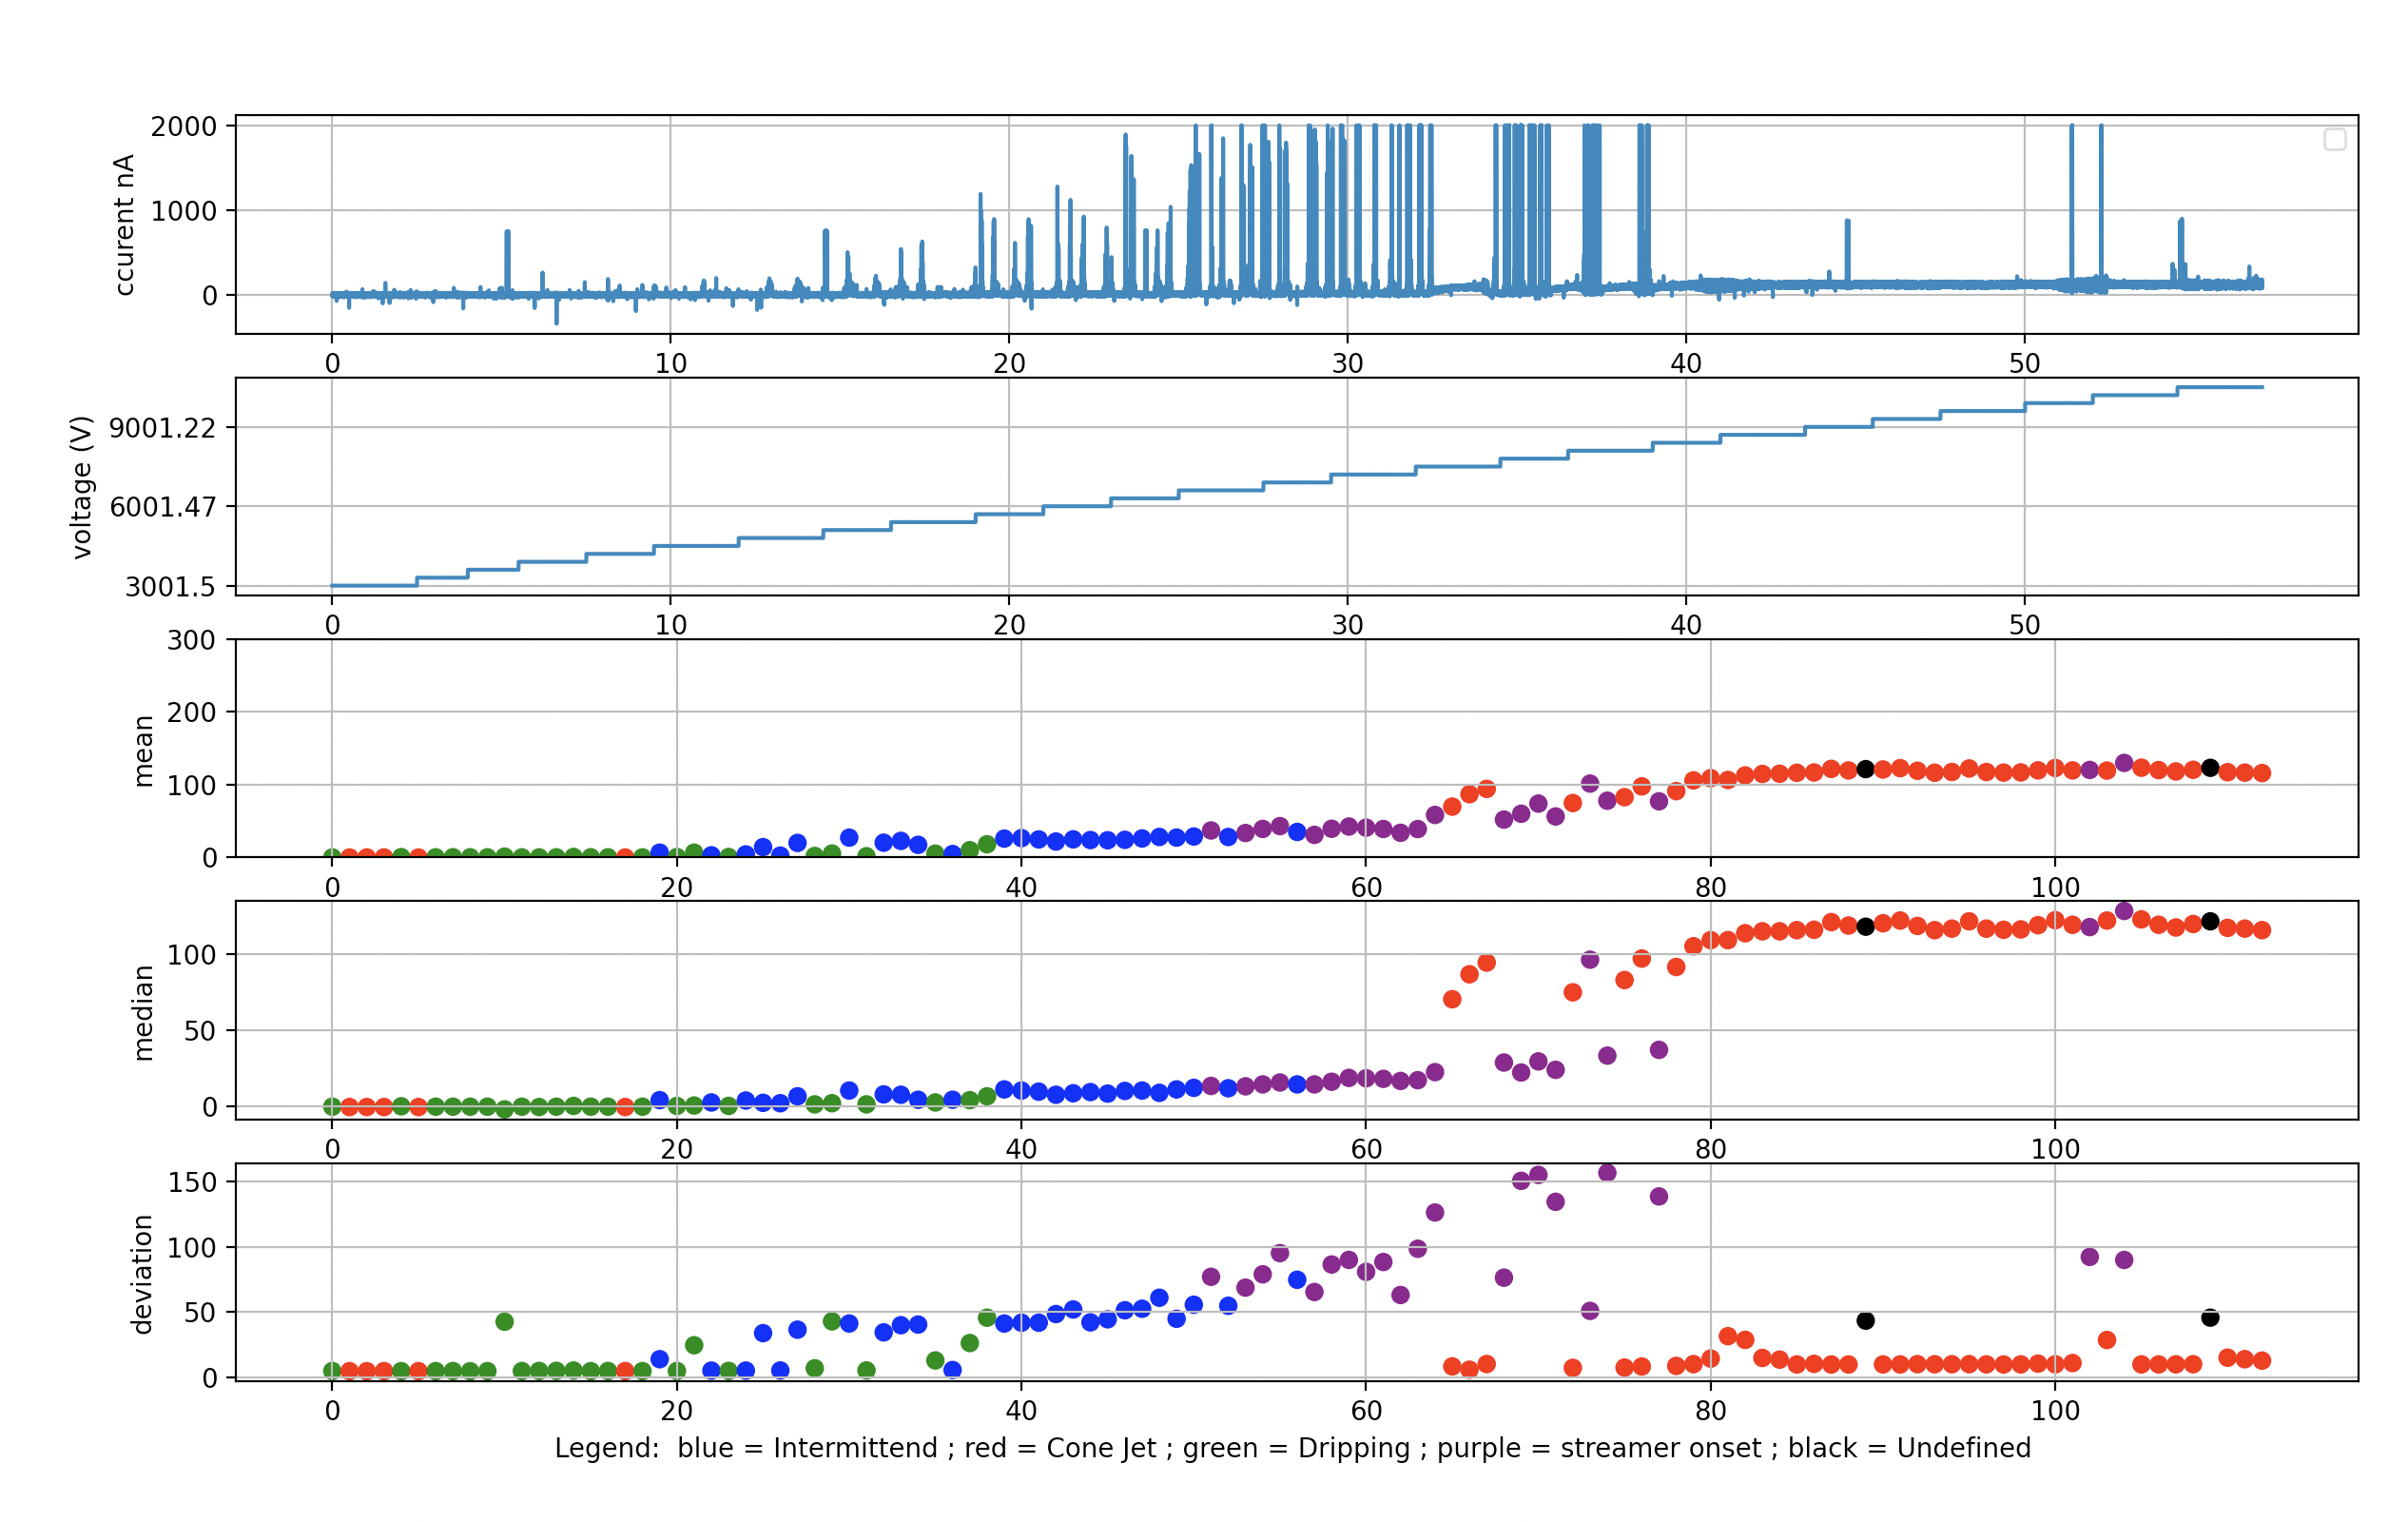
\includegraphics[width=18cm]{images/images_folder_2/img1.png}
    \caption{Data acquired in the experiment 1 - liquid: Water AND alcohol}
\end{figure}

\begin{figure}[H]
    \center
    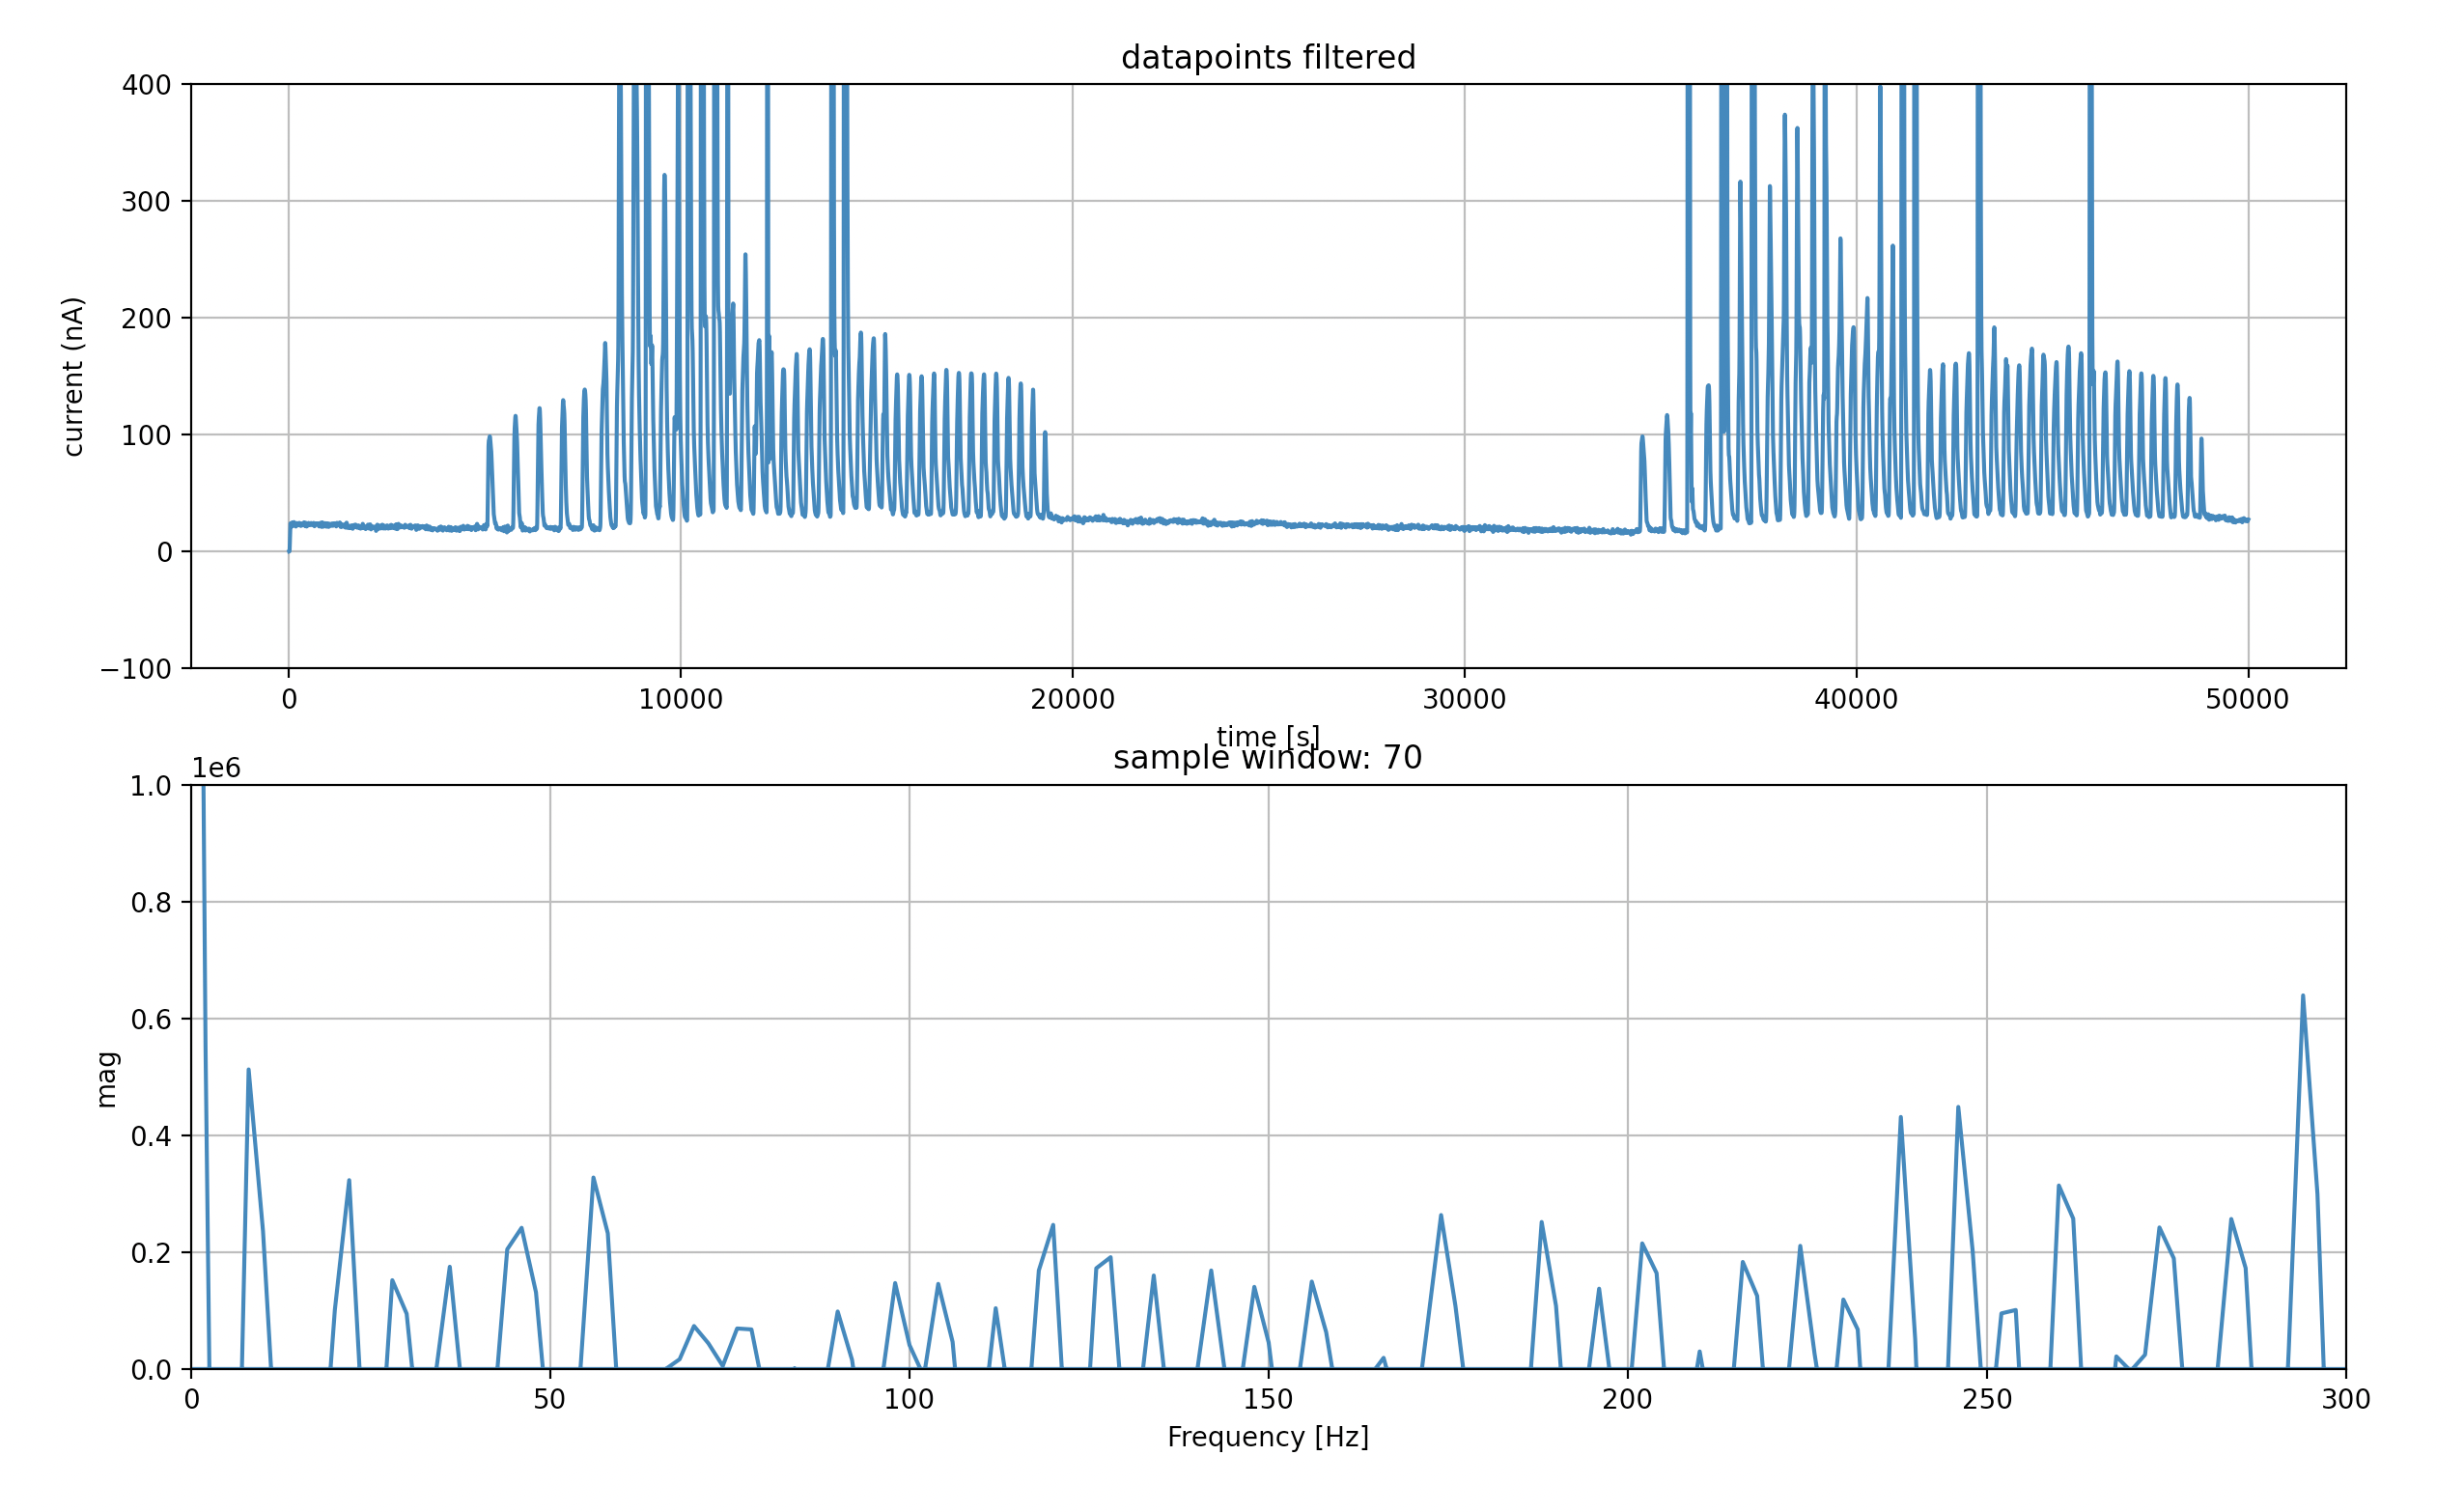
\includegraphics[width=12cm]{images/images_folder_2/img2.png}
    \caption{Dripping sample}
\end{figure}

\begin{figure}[H]
    \center
    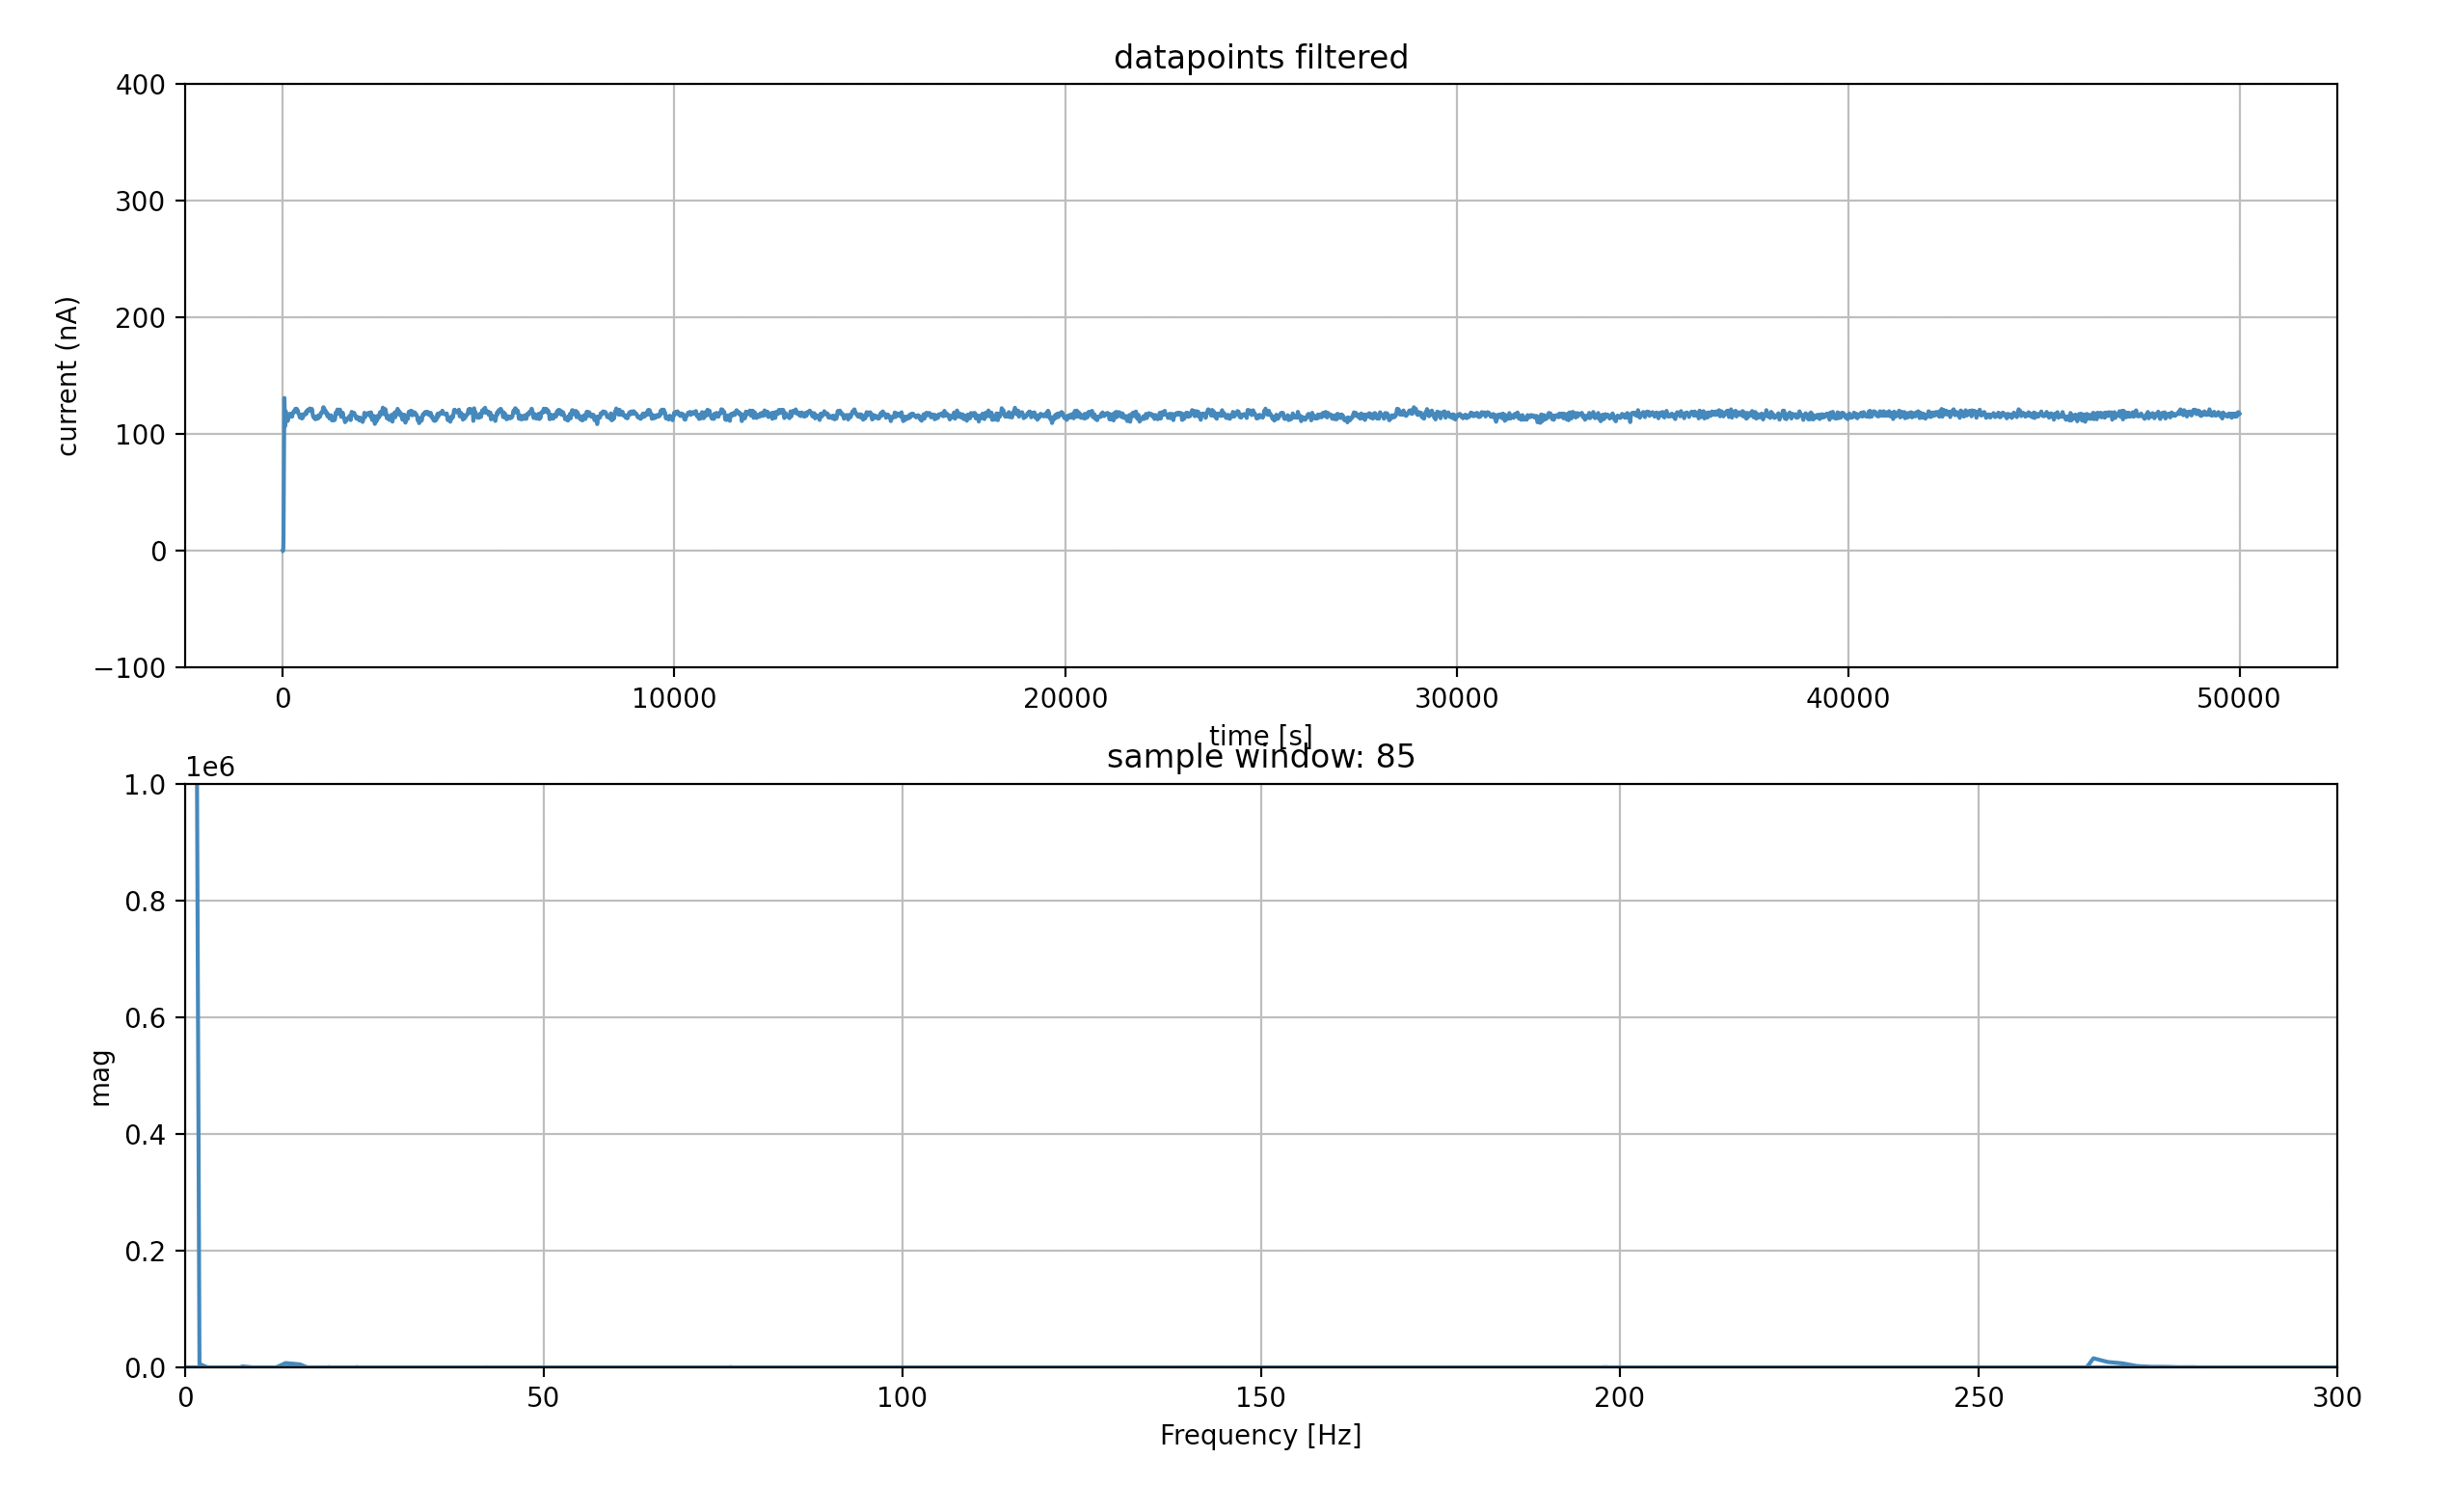
\includegraphics[width=15cm]{images/images_folder_2/img3.png}
    \caption{Cone jet sample}
\end{figure}

\begin{multicols}{3}

    \begin{figure}[H]
        \center
        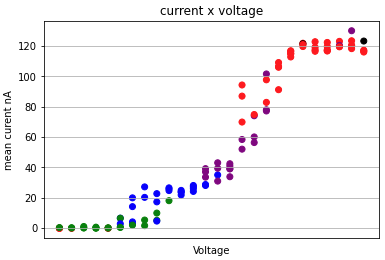
\includegraphics[width=5cm]{images/images_folder_3/data2_sjaaksgraph1.png}
        \caption{mean current X voltage}
    \end{figure}


    \begin{figure}[H]
        \center
        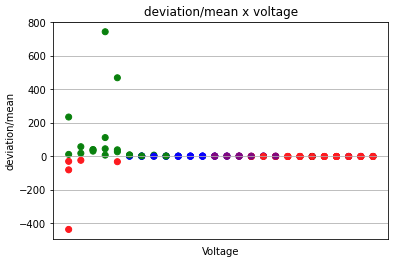
\includegraphics[width=5cm]{images/images_folder_3/data2_sjaaksgraph2.png}
        \caption{deviation/mean}
    \end{figure}


    \begin{figure}[H]
        \center
        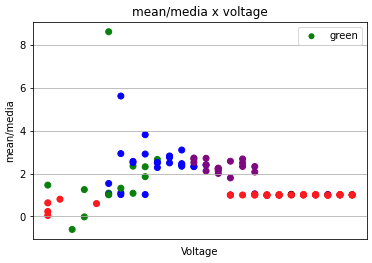
\includegraphics[width=5cm]{images/images_folder_3/data2_sjaaksgraph3.png}
        \caption{mean/median}
    \end{figure}

\end{multicols}

\subsection*{3.3 Experiment 2}

\begin{figure}[H]
    \center
    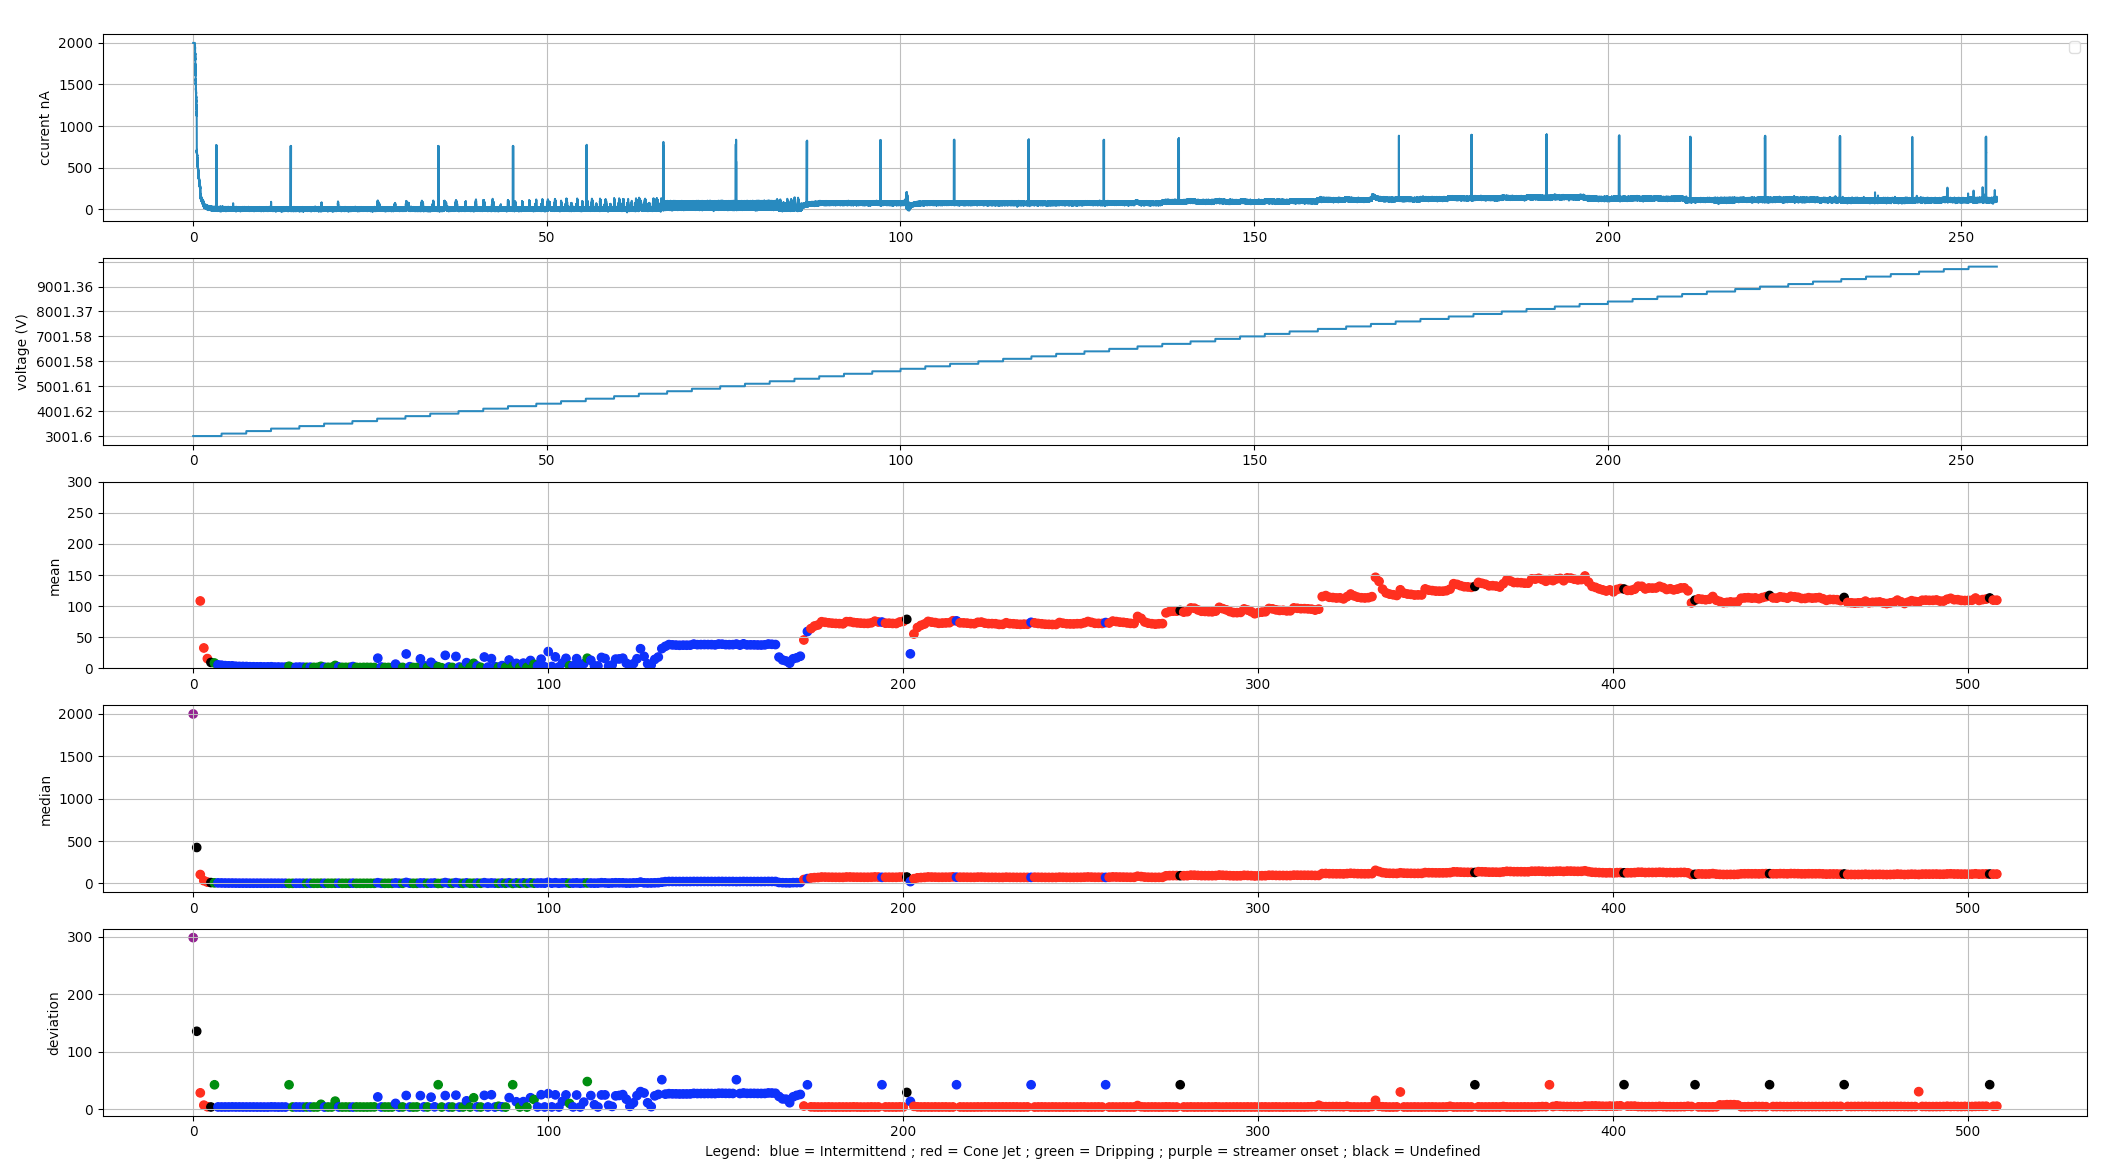
\includegraphics[width=18cm]{images/images_folder_3/data3.png}
    \caption{Data acquired in the experiment 2 - pure ethanol}
\end{figure}


\begin{figure}[H]
    \center
    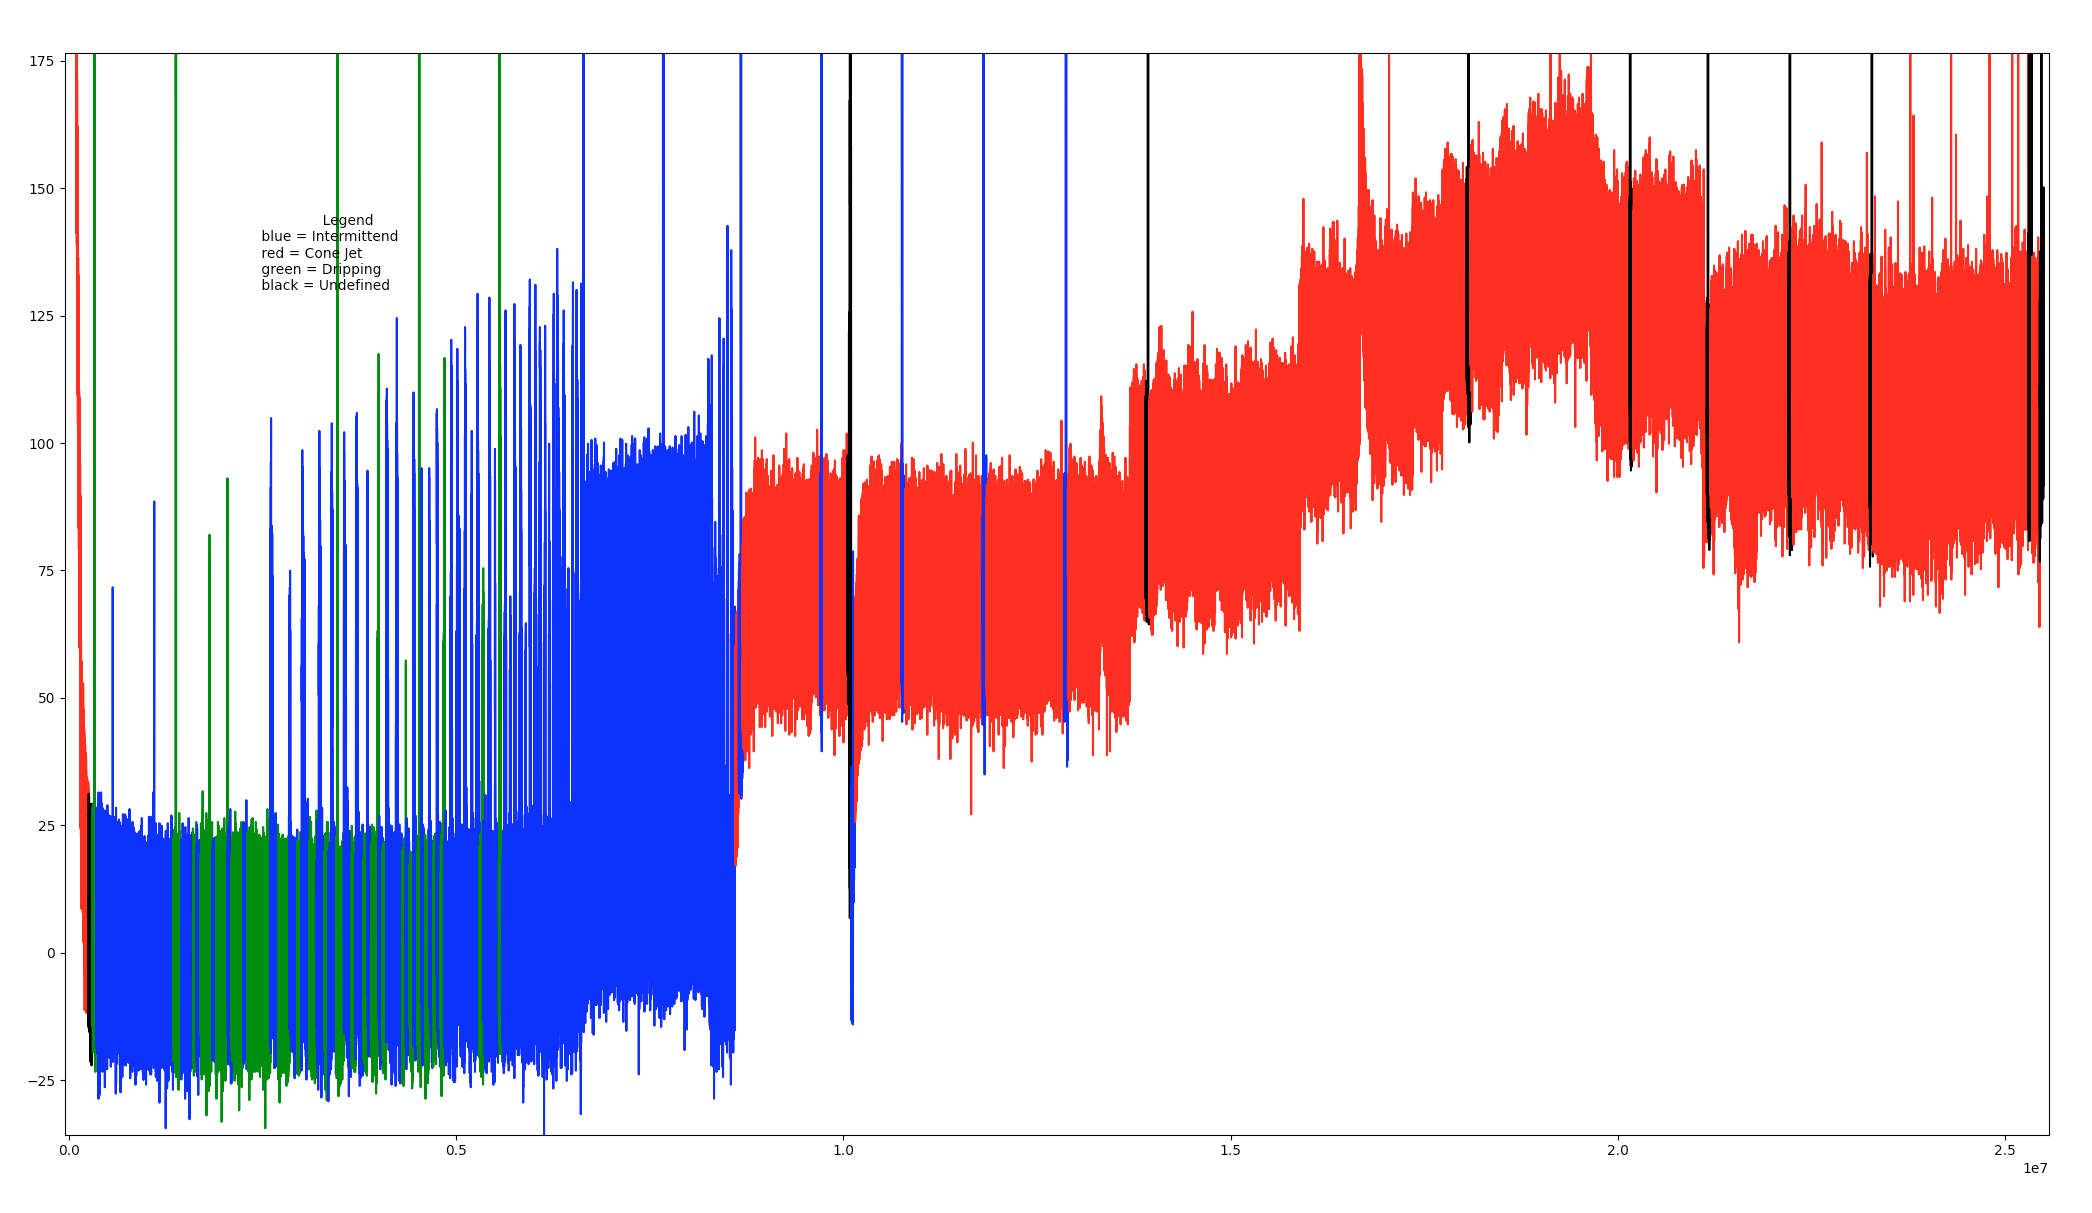
\includegraphics[width=12cm]{images/images_folder_3/data3current.png}
    \caption{current graph with classification}
\end{figure}

\begin{multicols}{3}

    \begin{figure}[H]
        \center
        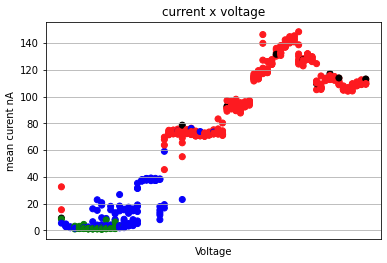
\includegraphics[width=5cm]{images/images_folder_3/data3_sjaaksgraph1.png}
        \caption{current mean X voltage}
    \end{figure}

    \begin{figure}[H]
        \center
        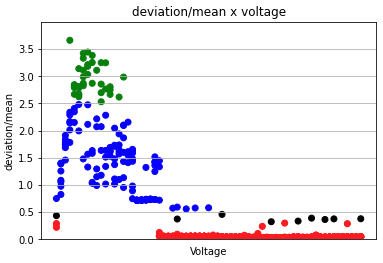
\includegraphics[width=5cm]{images/images_folder_3/data3_sjaaksgraph2.png}
        \caption{deviation/mean}
    \end{figure}

    \begin{figure}[H]
        \center
        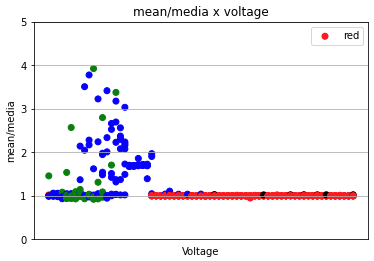
\includegraphics[width=5cm]{images/images_folder_3/data3_sjaaksgraph3.png}
        \caption{mean/median}
    \end{figure}

\end{multicols}


\subsection*{3.4 Experiment 3}

\begin{figure}[H]
    \center
    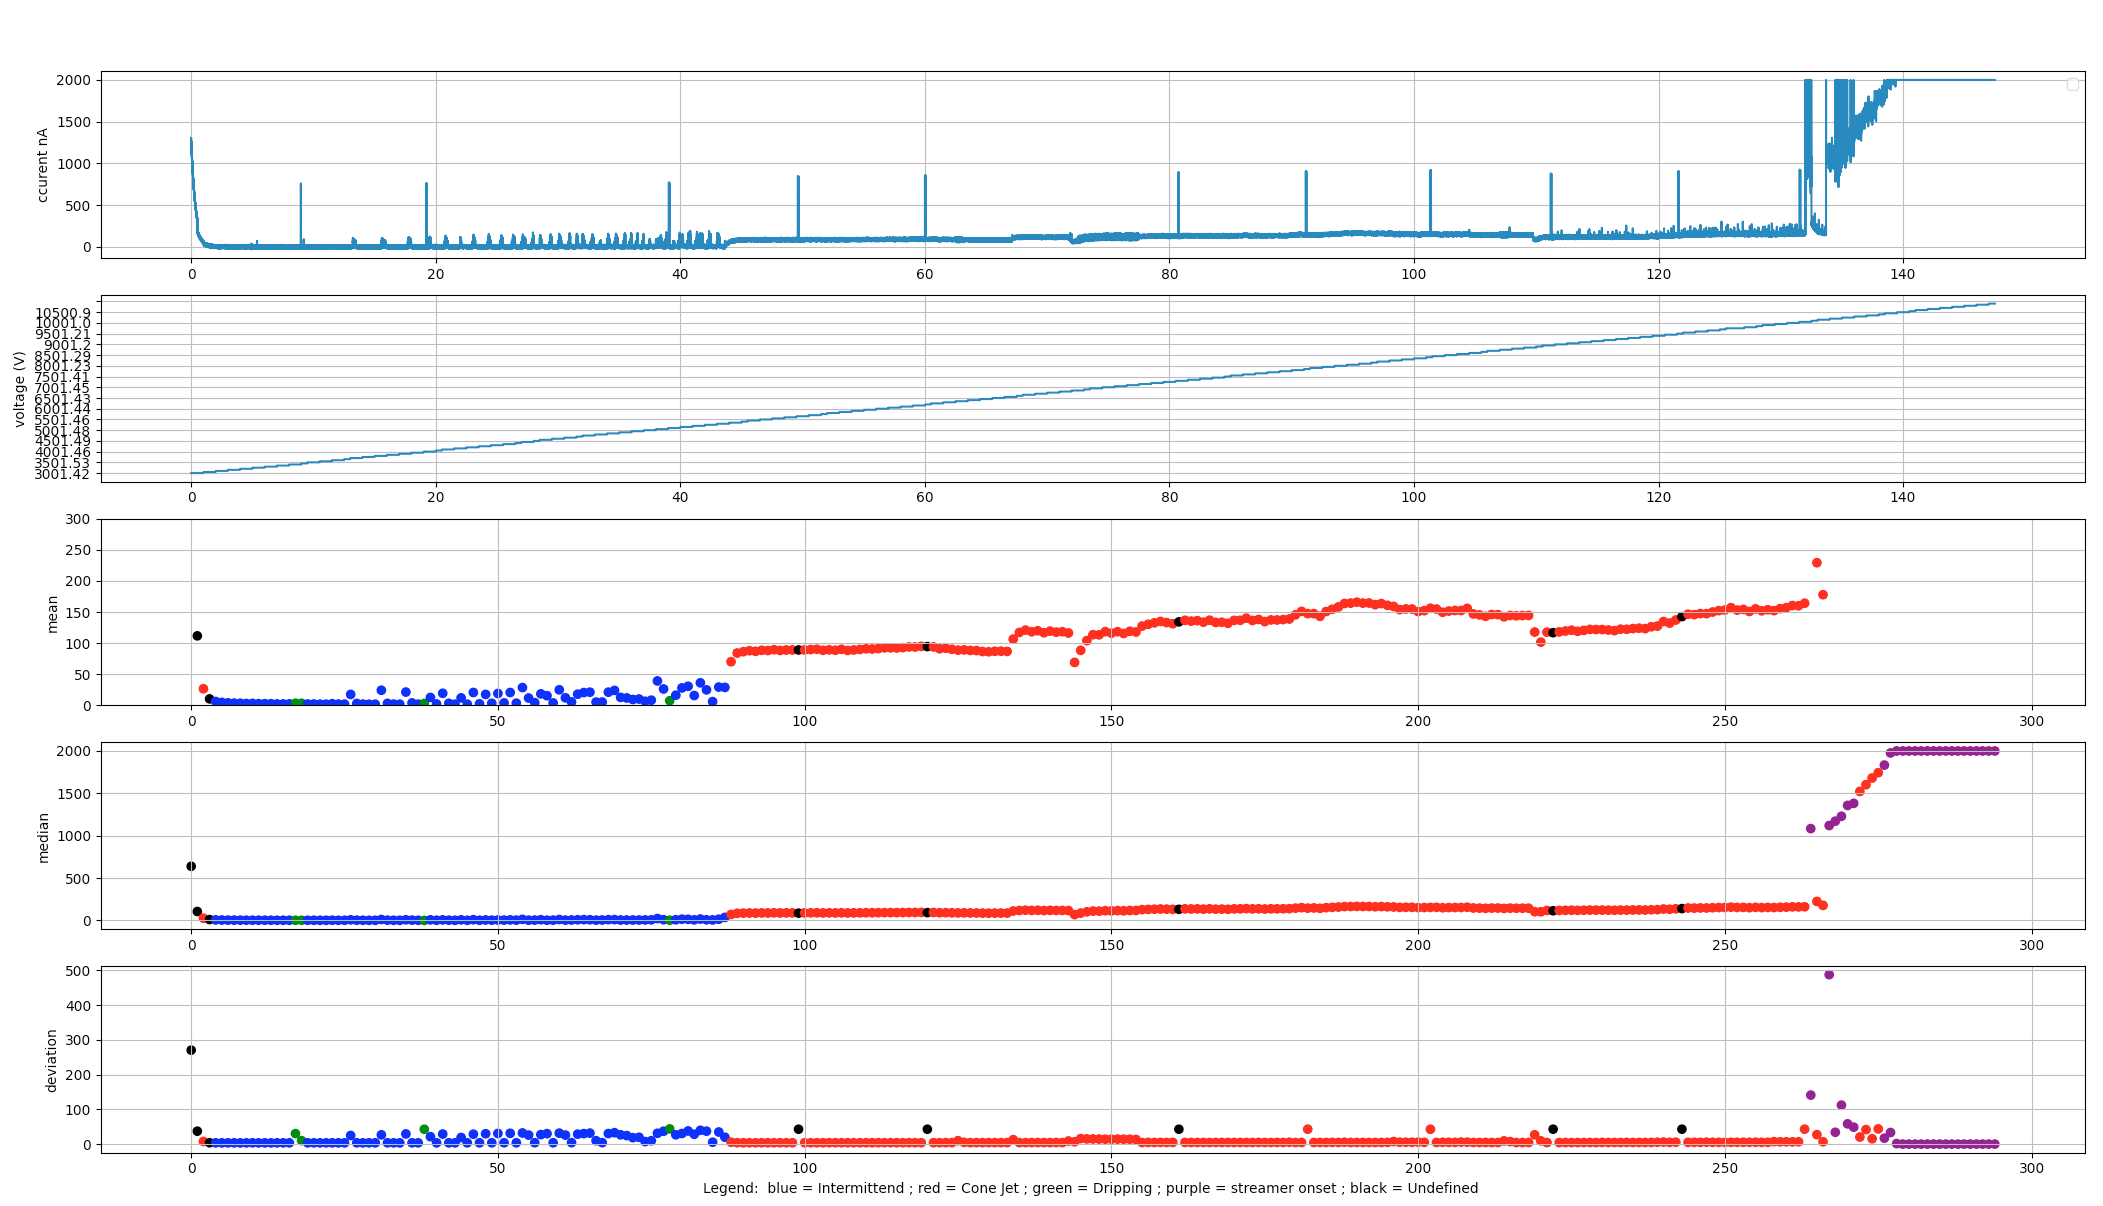
\includegraphics[width=18cm]{images/images_folder_3/data4.png}
    \caption{Data acquired in the experiment 3 - pure ethanol}
\end{figure}

\begin{multicols}{3}

    \begin{figure}[H]
        \center
        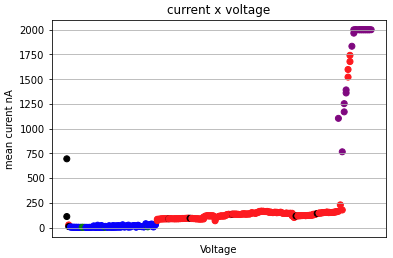
\includegraphics[width=5cm]{images/images_folder_3/data4_sjaakgraph1.png}
        \caption{current mean X voltage}
    \end{figure}

    \begin{figure}[H]
        \center
        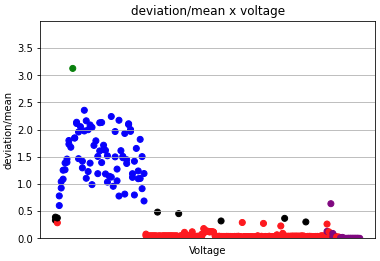
\includegraphics[width=5cm]{images/images_folder_3/data4_sjaakgraph2.png}
        \caption{deviation/mean}
    \end{figure}

    \begin{figure}[H]
        \center
        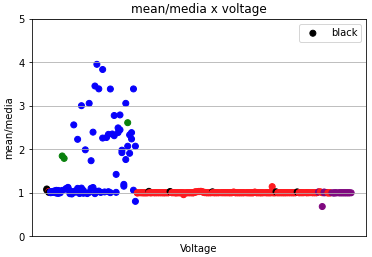
\includegraphics[width=5cm]{images/images_folder_3/data4_sjaakgraph3.png}
        \caption{mean/median}
    \end{figure}

\end{multicols}




